
\documentclass{vgtc}                          % final (conference style)
%\documentclass[review]{vgtc}                 % review
%\documentclass[widereview]{vgtc}             % wide-spaced review
%\documentclass[preprint]{vgtc}               % preprint
%\documentclass[electronic]{vgtc}             % electronic version

\usepackage{mathptmx}
\usepackage{graphicx}
\usepackage{times}
\usepackage{url}
\usepackage{epsfig}
\usepackage{psfrag}

%% We encourage the use of mathptmx for consistent usage of times font
%% throughout the proceedings. However, if you encounter conflicts
%% with other math-related packages, you may want to disable it.

%% If you are submitting a paper to a conference for review with a double
%% blind reviewing process, please replace the value ``0'' below with your
%% OnlineID. Otherwise, you may safely leave it at ``0''.
\onlineid{0}

%% declare the category of your paper, only shown in review mode
\vgtccategory{Research}

%% allow for this line if you want the electronic option to work properly
\vgtcinsertpkg

%% In preprint mode you may define your own headline.
%\preprinttext{To appear in an IEEE VGTC sponsored conference.}

%% Paper title.

\title{Interactive Multiplots For Comparing Coverage Effectiveness}

%% Author and Affiliation (multiple authors with single affiliations).
%%\author{Roy G. Biv\thanks{e-mail: roy.g.biv@aol.com} %
%%\and Ed Grimley\thanks{e-mail:ed.grimley@aol.com} %
%%\and Martha Stewart\thanks{e-mail:martha.stewart@marthastewart.com}}
%%\affiliation{\scriptsize Martha Stewart Enterprises \\ Microsoft Research}

%% Author and Affiliation (multiple authors with multiple affiliations)
\author{Adam M. Smith\thanks{e-mail: ams292@cs.pitt.edu} %
\and Joshua J. Geiger\thanks{e-mail:jj55@cs.pitt.edu}} %
\affiliation{\scriptsize University of Pittsburgh}


\abstract{Software testing increases confidence in the correctness of an application's source code.  Altering a test suite's execution order enables earlier detection of defects and allows developers to fix errors sooner.  The many existing ordering methods produce different possible test suite orders to choose from.  This paper presents tool support for a technique that allows for a comparison of test suite orders through visualization and interaction.}

%% ACM Computing Classification System (CCS). 
%% See <http://www.acm.org/class/1998/> for details.
%% The ``\CCScat'' command takes four arguments.

%%\CCScatlist{ 
 %% \CCScat{K.6.1}{Management of Computing and Information Systems}%
%%{Project and People Management}{Life Cycle};
%%  \CCScat{K.7.m}{The Computing Profession}{Miscellaneous}{Ethics}
%%}

%% Copyright space is enabled by default as required by guidelines.
%% It is disabled by the 'review' option or via the following command:
% \nocopyrightspace

%%%%%%%%%%%%%%%%%%%%%%%%%%%%%%%%%%%%%%%%%%%%%%%%%%%%%%%%%%%%%%%%
%%%%%%%%%%%%%%%%%%%%%% START OF THE PAPER %%%%%%%%%%%%%%%%%%%%%%
%%%%%%%%%%%%%%%%%%%%%%%%%%%%%%%%%%%%%%%%%%%%%%%%%%%%%%%%%%%%%%%%%

\begin{document}

%% The ``\maketitle'' command must be the first command after the
%% ``\begin{document}'' command. It prepares and prints the title block.

%% the only exception to this rule is the \firstsection command
\firstsection{Introduction}

\maketitle

%% \section{Introduction} 

Developers inevitably create errors while designing and implementing software systems. Software developers execute tests $\langle t_1, t_2, t_3,\ldots, t_n\rangle$ in a test suite $T$ to isolate defects and gain confidence in the correctness of the code.  Each test case in the test suite exercises specific points in the system, comparing the actual output of the code to the hand computed expected one.  If a test fails then it is likely that a defect is present in the source code that the test executes.  As the source code grows in size and number of features new tests are written for the new functionality.  To ensure that the new features do not cause the system to regress, developers include every previously written test in the collection of tests.  This process of executing and re-executing the entire test suite is known as regression testing.  

Gradually, adding new tests and retaining old ones increases the size of the test suite until its execution time can become prohibitively expensive.  In some cases the regression test suite runs for several weeks \cite{empiricalfamily}.  One method of altering the test suite to resolve this issue is test suite prioritization \cite{rothermelprioritizing2001}.  Prioritization attempts to find an ordering of the test cases that is more likely to locate defaults earlier in the execution of the test suite without risking the loss of coverage by removing a test.  The tests are ordered based on certain criteria that are obtained during a process called coverage monitoring.  

Coverage monitoring measures the code coverage of a test case $t_i$.  Code coverage describes any metric that enumerates specific points in the source code that are executed when a test is run, whether they are a line, a block, a method, a branch \cite{zhu}, call trees \cite{smith:2007}, or some other type. Each specific program point is called a requirement.  Given a test suite $T$, coverage monitoring gives a set of requirements $R(T) = \{ r_1, r_2,\ldots,r_m \}$.  Each individual test $t_i$ is associated with a subset of requirements $R(t_i) \subseteq R(T)$, which it is said to \textit{cover}.  

\begin{figure}[t]
\centering
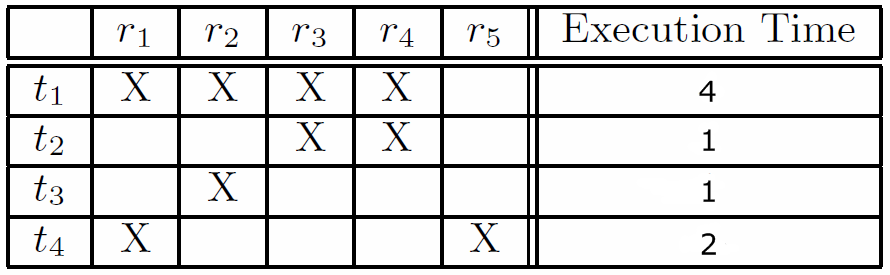
\includegraphics[scale=.2]{CoverageMatrix.png}
\caption{Example Test Suite}
\end{figure}
\label{fig:example}

\begin{figure}[t]
\centering

\psfrag{tone1059}[cc][cc]{$t_1$ Done}
\psfrag{tone1060}[cc][cc]{$t_{n-1}$ Done}
\psfrag{tone1061}[cc][cc]{$t_{n}$ Done}
\psfrag{cover1059}[cc][cc]{$\;\;$ Cover $\cal{R}$$(t_1)$}
\psfrag{cover1060}[cc][cc]{Cover $\bigcup_{i = 1}^{n-1}$$ \cal{R}$$(t_i)$}
\psfrag{cover1061}[cc][cc]{\hspace{10pt} Cover $\cal{R}$$(T)$}
\psfrag{area1061}[cc][cc]{\hspace{10pt} Area $\int_0^{l(n)} \mathrm{C}(T, l)$}
\psfrag{ccTc}[cc][cc]{${\scriptstyle \mathrm{C}(T,l)}$}
\psfrag{ttTt}[cc][cc]{$(l)$}

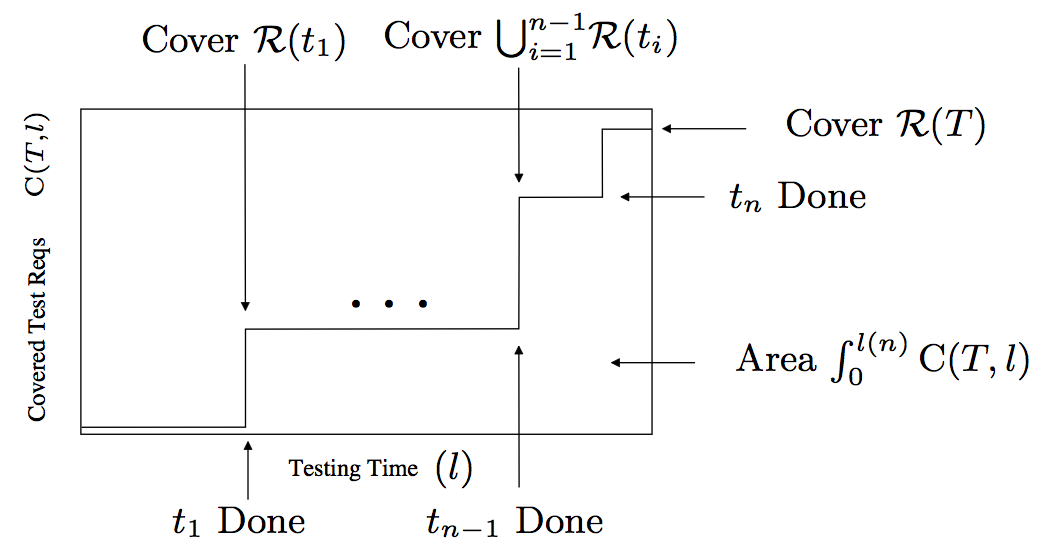
\includegraphics[width=3in]{cum_cov_final.png}
\vspace{.05in}
\caption{Coverage Effectiveness.} %\cite{ce} (Used with permission of author).} % can't cite in captions apparently.
\vspace{-.2in}
\label{fig:ce}
\end{figure}	

%\begin{figure}[ht]
%\centering
%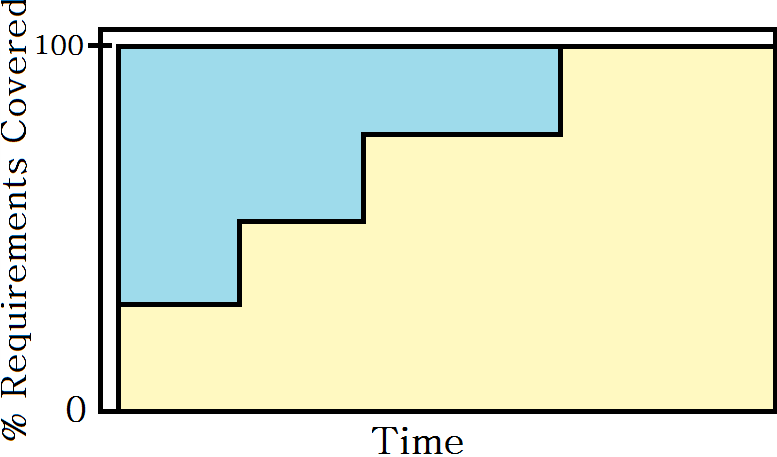
\includegraphics[scale=.2]{ce}
%\caption{Coverage Effectiveness}
%\end{figure}
%\label{fig:ce}

Figure \ref{fig:example} shows an example of a test suite with 4 tests and 5 requirements.  An X in a cell represents that the test for that row covers the requirement in that column.  Consider running the shown test suite in its original order.  In this case all of the requirements are not covered until 8 time units have passed.  Conversely, if the test suite is executed in reverse order all of the requirements are covered in 4 time units.  Covering all of the requirements sooner allows for a higher chance to find faults earlier so that the developer can more quickly begin to make changes.

The metric coverage effectiveness (CE) \cite{ce} was developed in order to rate a test suite prioritization.  CE is derived from the step function of the cumulative coverage of a test suite as shown in Figure \ref{fig:ce}.  Each test suite offers the possibility of covering more total requirements.  When the cumulative coverage is plotted against time a step function is formed.  CE itself is calculated by dividing the area under the step function for the actual order by the area under the curve of a test suite that covers all of its requirements instantly.  This value is inclusively between 0 and and less than 1 where a CE of 0 would mean that no requirements were covered and a CE of 1 would mean that all of the requirements were covered instantly.

\section{Motivation}

For test suites with $n$ tests it is too expensive to generate all $n!\!$ possible orderings to find the best CE value.  For this reason there are several algorithms that prioritize test suites.  Given coverage and timing data for a test suite this tool generates several prioritizations using the implementations of greedy (GRD), 2-optimal greedy (2OPT), delayed greedy (DGR), and Harrold Gupta Soffa (HGS) algorithms described in Smith and Kapfhammer \cite{smith:2009}.  These algorithms can use the execution time (cost), covered requirements (coverage), or a ratio of covered requirements per unit time (ratio) to make all necessary greedy choices.

% This paragraph needs work.
In addition to algorithmic approaches to prioritization, random sampling may produce orderings that are favored over the original order.  Generating large random samples also gives insight into the difficulty of finding a good ordering.  The reverse order of a test suite also tends to produce higher CE values than the original. %need to cite rothermel i think. \cite{{} 

It is difficult to interpret the results of several algorithms or random samples by reading text alone.  Therefore, this paper presents a visualization that can allow software testers to examine a large set of test suite orders simultaneously.   Related work in the field of visualizing test suites exists \cite{bart} \cite{tarantula}, however, it focuses on fault localization or different features of a test suite.

Examining the CE functions of several orderings for a given test suite will reveal the effectiveness of the different prioritization techniques on that suite.  Figure \ref{fig:multi_ce} shows a multiplot of CE functions for 50 random prioritizations.  This static image does not allow for easy identification of the source of the prioritizations.  Also, the static image cannot display qualitative data without using a large legend.  To allow for more information communication the visualization provides interactivity in order to more easily allow test suite orders to be compared.

\begin{figure}[t]
\centering
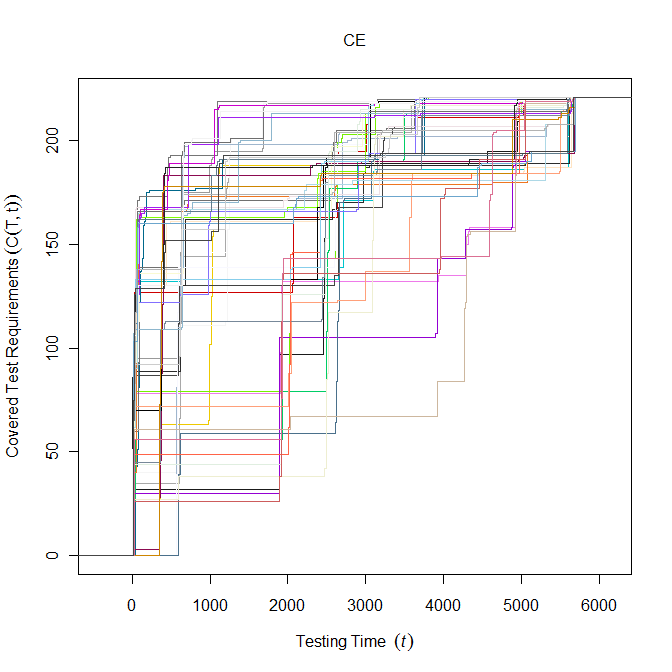
\includegraphics[scale=.25]{original.png}
\caption{Coverage Effectiveness Multiplot}
\end{figure}
\label{fig:multi_ce}

\section{Tool Design}

The tool is designed to aid in analyzing multiple prioritizations of a test suite through user interaction of CE multiplots. Due to the fact that step functions consist of only vertical and horizontal lines, plotting several functions on a single graph may obscure lines, thus making it difficult to track and compare prioritizations.  A solution to this is pruning the graph to only the plots in which the user is interested.  However, generating a new static multiplot for each comparison is cumbersome.  Therefore, in a similar approach to Becker et al$.$ \cite{Stephen95visualizingnetwork} and a NY Times interactive visualization of market statstics \cite{nytime_multiplot} the tool allows users to interactively select techniques displayed and directly manipulate the corresponding plot.  Figure \ref{fig:screenshot} provides a screen capture of the tool.  

The left panel provides information about the test suite and allows the user to select which technique's results will be displayed in the multiplot.  The first set of buttons will display the original or the reverse order of the test suite.  The button matrix toggles displaying the results of the prioritization algorithms introduced above.  Each row represents a prioritization technique and each column shows a greedy choice metric.  To display the results of a technique given a specific metric the user may click on the appropriate cell in the matrix.  Each technique button is color coded to match its step function line in the plot for easy identification.  The slider bar allows the user to choose a number of random prioritizations that are displayed in the plot as thinner gray lines.  

%need to add to this as well.
The right panel displays the multiplot.   In this image, all techniques are currently selected to appear in the multiplot.  A mouseover on a function line highlights it and shades the area under it, as well as, provide a label identfying the technique, greedy choice metric, and the CE value of the prioritization represented by the line.  

\section{Evaluation}

%Feedback on the usability and effectiveness in aiding CE comparisons of the tool was primarily provided by Dr. Gregory M. Kapfhammer, an expert in software engineering, software testing and analysis, and computer systems \cite{thehammer}.  Response to the tool was generally positive, the evaluator found the tool useful in displaying the information but made suggestions on areas where the tool could help to interpret the data.  Some suggestions include:
%\begin{itemize}
% \item Displaying coverage density information
% \item Relate 'goodness' of approach (CE) through glyphs or colors
% \item Empirical cumulative distribution functions of the random
% \end{itemize}
%A few other suggestions on layout were also made, but our evaluator stated that the tool was already useful enough that he would use it in his own research, as well as, utilize it in teaching his future software engineering courses.  Overall, the tool met its goal of providing simple interactive technique for comparing prioritization effectiveness.

\begin{figure}
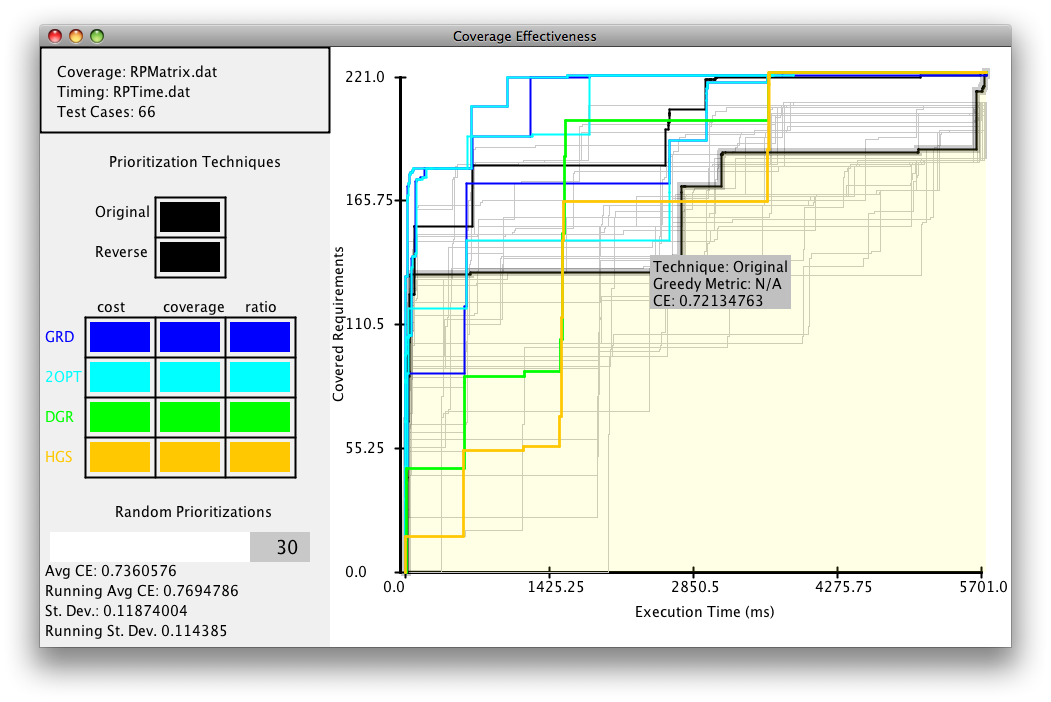
\includegraphics[scale=.25]{screenshot.png}
\caption{Interactive Multiplot}
\label{fig:screenshot}
\end{figure}

%% if specified like this the section will be ommitted in review mode
\acknowledgements{
The authors wish to thank Gregory Kapfhammer, Manos Renieris, and Liz Marai for assistance with this project.}

\bibliographystyle{abbrv}
%%use following if all content of bibtex file should be shown
%\nocite{*}
\bibliography{myBibtexDB}
\end{document}
